% ---------------------------------------------------------------------
% EG author guidelines plus sample file for EG publication using LaTeX2e input
% D.Fellner, v2.02, Jan 25, 2017


\title[Seminar Topic]%
      {Graph Layouting for Visualizing Graph Structured Data}

% for anonymous conference submission please enter your SUBMISSION ID
% instead of the author's name (and leave the affiliation blank) !!
\author[M.Rosier \& K.\"ohlein]
{\parbox{\textwidth}{\centering Marcel Rosier$^1$% 
\\ Seminar: Data Visualization %
\\ marcel.rosier@tum.de% 
\\ Supervisor: Kevin H\"ohlein%
%        S. Spencer$^2$\thanks{Chairman Siggraph Publications Board}
        }
        \\
% For Computer Graphics Forum: Please use the abbreviation of your first name.
{\parbox{\textwidth}{\centering $^1$ Technische Universit\"at M\"unchen
%        $^2$ Another Department to illustrate the use in papers from authors
%             with different affiliations
       }
}
}
% ------------------------------------------------------------------------

% if the Editors-in-Chief have given you the data, you may uncomment
% the following five lines and insert it here
%
% \volume{36}   % the volume in which the issue will be published;
% \issue{1}     % the issue number of the publication
% \pStartPage{1}      % set starting page


%-------------------------------------------------------------------------
\begin{document}

\teaser{
 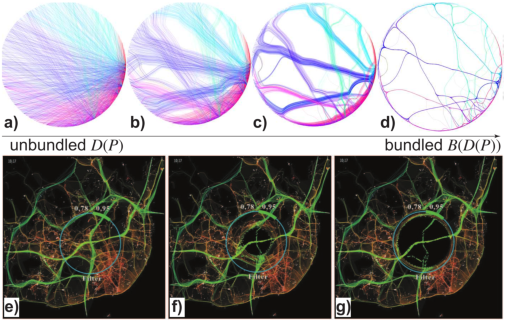
\includegraphics[width=\linewidth]{media/teaser.pdf}
 \centering
  \caption{Four frames from a global edge bundle relaxation process. The bundling tightness increases from a to d. Taken from \cite{Lhuillier2017}.  }
\label{fig:teaser}
}

\maketitle
%-------------------------------------------------------------------------
\begin{abstract}
Graph structured data can be found in biology, social networks and various other modern applications. To get an overview of this data and extract relevant information from it a fitting visualization is necessary. Although basic graph drawing has been a research topic for a long time, the underlying graphs have grown to a scale, at which modern applications deal with huge graph structures that contain millions of nodes and edges.
Therefore finding appropriate layouts and reasonable simplification techniques becomes more and more relevant. This paper provides an overview of basic graph representations, layouting and complexity reduction techniques as well as common user interaction methods. A special focus is given to the complexity reduction approach edge bundling. 

%-------------------------------------------------------------------------
%  ACM CCS 1998
%  (see http://www.acm.org/about/class/1998)
% \begin{classification} % according to http:http://www.acm.org/about/class/1998
% \CCScat{Computer Graphics}{I.3.3}{Picture/Image Generation}{Line and curve generation}
% \end{classification}
%-------------------------------------------------------------------------


\end{abstract}  
%-------------------------------------------------------------------------
\section{Introduction}
A graph is mathematically defined as a tuple $ G = (V, E)$ with $V$ being a set of vertices (often also referred to as nodes) and $E \subseteq V^2$ being a set of edges \cite{Al-Taie2017}. In the context of using graphs for data representation each edge describes a relation between two nodes and can be either directed or undirected. A sequence of edges along distinct vertices is called a path. Moreover, edges and vertices can have attributes, that provide additional information about them. A connected acyclic graph is called a tree. Graphs can also be time dependent and modifiable, e.g. through user interaction. These graphs are called dynamic. Visualizing dynamic graphs, however, is a topic on its own and beyond the scope of this paper.\\
\\
% Graphs come in various forms: Reaching from simple hierarchical Trees, e.g. in a file system, to gigantic graphs with millions of nodes and edges, for instance a social network.
In various areas - such as biology, software engineering or the analysis of social networks - graphs are a typical way of representing data. In order to analyze the contained information, it is insightful to visualize it. Therefore the mathematical concept of a graph needs to be mapped to a visual representation. This process isn't trivial since in many applications there may not be a natural way of mapping graphs with potentially high-dimensional and abstract node and edge properties to 2- or 3-dimensional visual representations.
The procedure of mapping a graph to a usually 2 or 3-dimensional area is called graph layouting. 
Considering the size of typical graphs that can quickly exceed thousands of nodes and edges - for example, a graph representing a social network like facebook -  the layout of a graph has a huge impact on understanding the local and global structure, connections and other analysis tasks. Thus layout techniques try to maximize readability by taking different aesthetic criteria into account. To improve readability the graph can be reduced in its complexity. Typical methods are for instance filtering, grouping or edge bundling (e.g. \autoref{fig:teaser}) which can be applied algorithmically, manually through user interactions or combined. \\ This paper is organized as follows: Section 2 gives an overview of possible visual representations of a graph and different families of layouting algorithms. In section 3 state of the art complexity reduction strategies are explained with a focus on edge bundling techniques and section 4 outlines common user interaction methods. Finally, section 5 summarizes the main aspects and points to open research topics.

\section{Visual Representation}
\subsection{Visualization options and criteria}
This paper will focus on two types of graph visualizations: node-link diagrams and adjacency matrices.
Node-link diagrams map nodes to positions and edges to links between the node positions. Positioning the nodes and drawing the links in an appropriate way, e.g. minimize edge crossings, is challenging. Adjacency matrices on the other side don't have issues with edge crossings. In this approach, a graph with $N$ vertices is visualized by an $N \times N $ matrix, in which every entry represents the edge between the vertices of the corresponding row and column. To improve readability an optimized node order has to be calculated, the edges are then implicitly displayed \cite{VonLandesberger2011}.\\
Both types have certain benefits: In a direct comparison node-link diagrams are more intuitive, compact and make it easier to follow paths but can be hard to understand due to problematic layouts. Adjacency matrices contrarily provide an uncluttered view for dense graphs but have issues displaying large networks \cite{Ghoniem2004}. Some approaches also combine the two types to synthesize their advantages. Examples for all mentioned options can be found in \autoref{fig:vis_types}.
\\\\
Most of the techniques introduced in this paper use node-link diagrams. This visualization style has infinitely many representations for the same graph that differ in readability. Therefore criteria that define a good layout are necessary to, later on, guide layouting techniques to good results. While many exist that each benefit the visualization of certain graphs, a few guidelines are common and work well on most graphs: \\
For instance, nodes should be evenly distributed and vertices that are similar with respect to attributes or edges should be clustered. Uniform edge lengths, minimal edge crossings and bends as well as an overall symmetric layout are also favorable \cite{Bennett2007}. \\
While all of these goals contribute to a good layout, its often impossible to achieve all of them simultaneously since they are competing with each other\cite{Gibson2013}. Hence a few criteria have to be prioritized and as a result different layout techniques focus on different goals.
%or even ignore them altogether.
In the following subsection, a selection of layout algorithms classified by their node placement will be introduced and shortly reviewed.
% This representation provides an intuitive overview and allows users to easily follow paths \cite{}
\begin{figure}
    \centering
    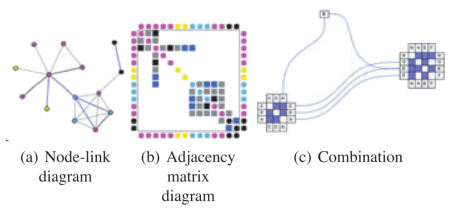
\includegraphics[width=\linewidth]{media/vis_types.pdf}
    \caption{Three common types of graph visualization techniques (node-link, adjacency matrix and a combination) applied to the same graph. Taken from \cite{VonLandesberger2011}.}
    \label{fig:vis_types}
\end{figure}

\begin{figure}
    \centering
    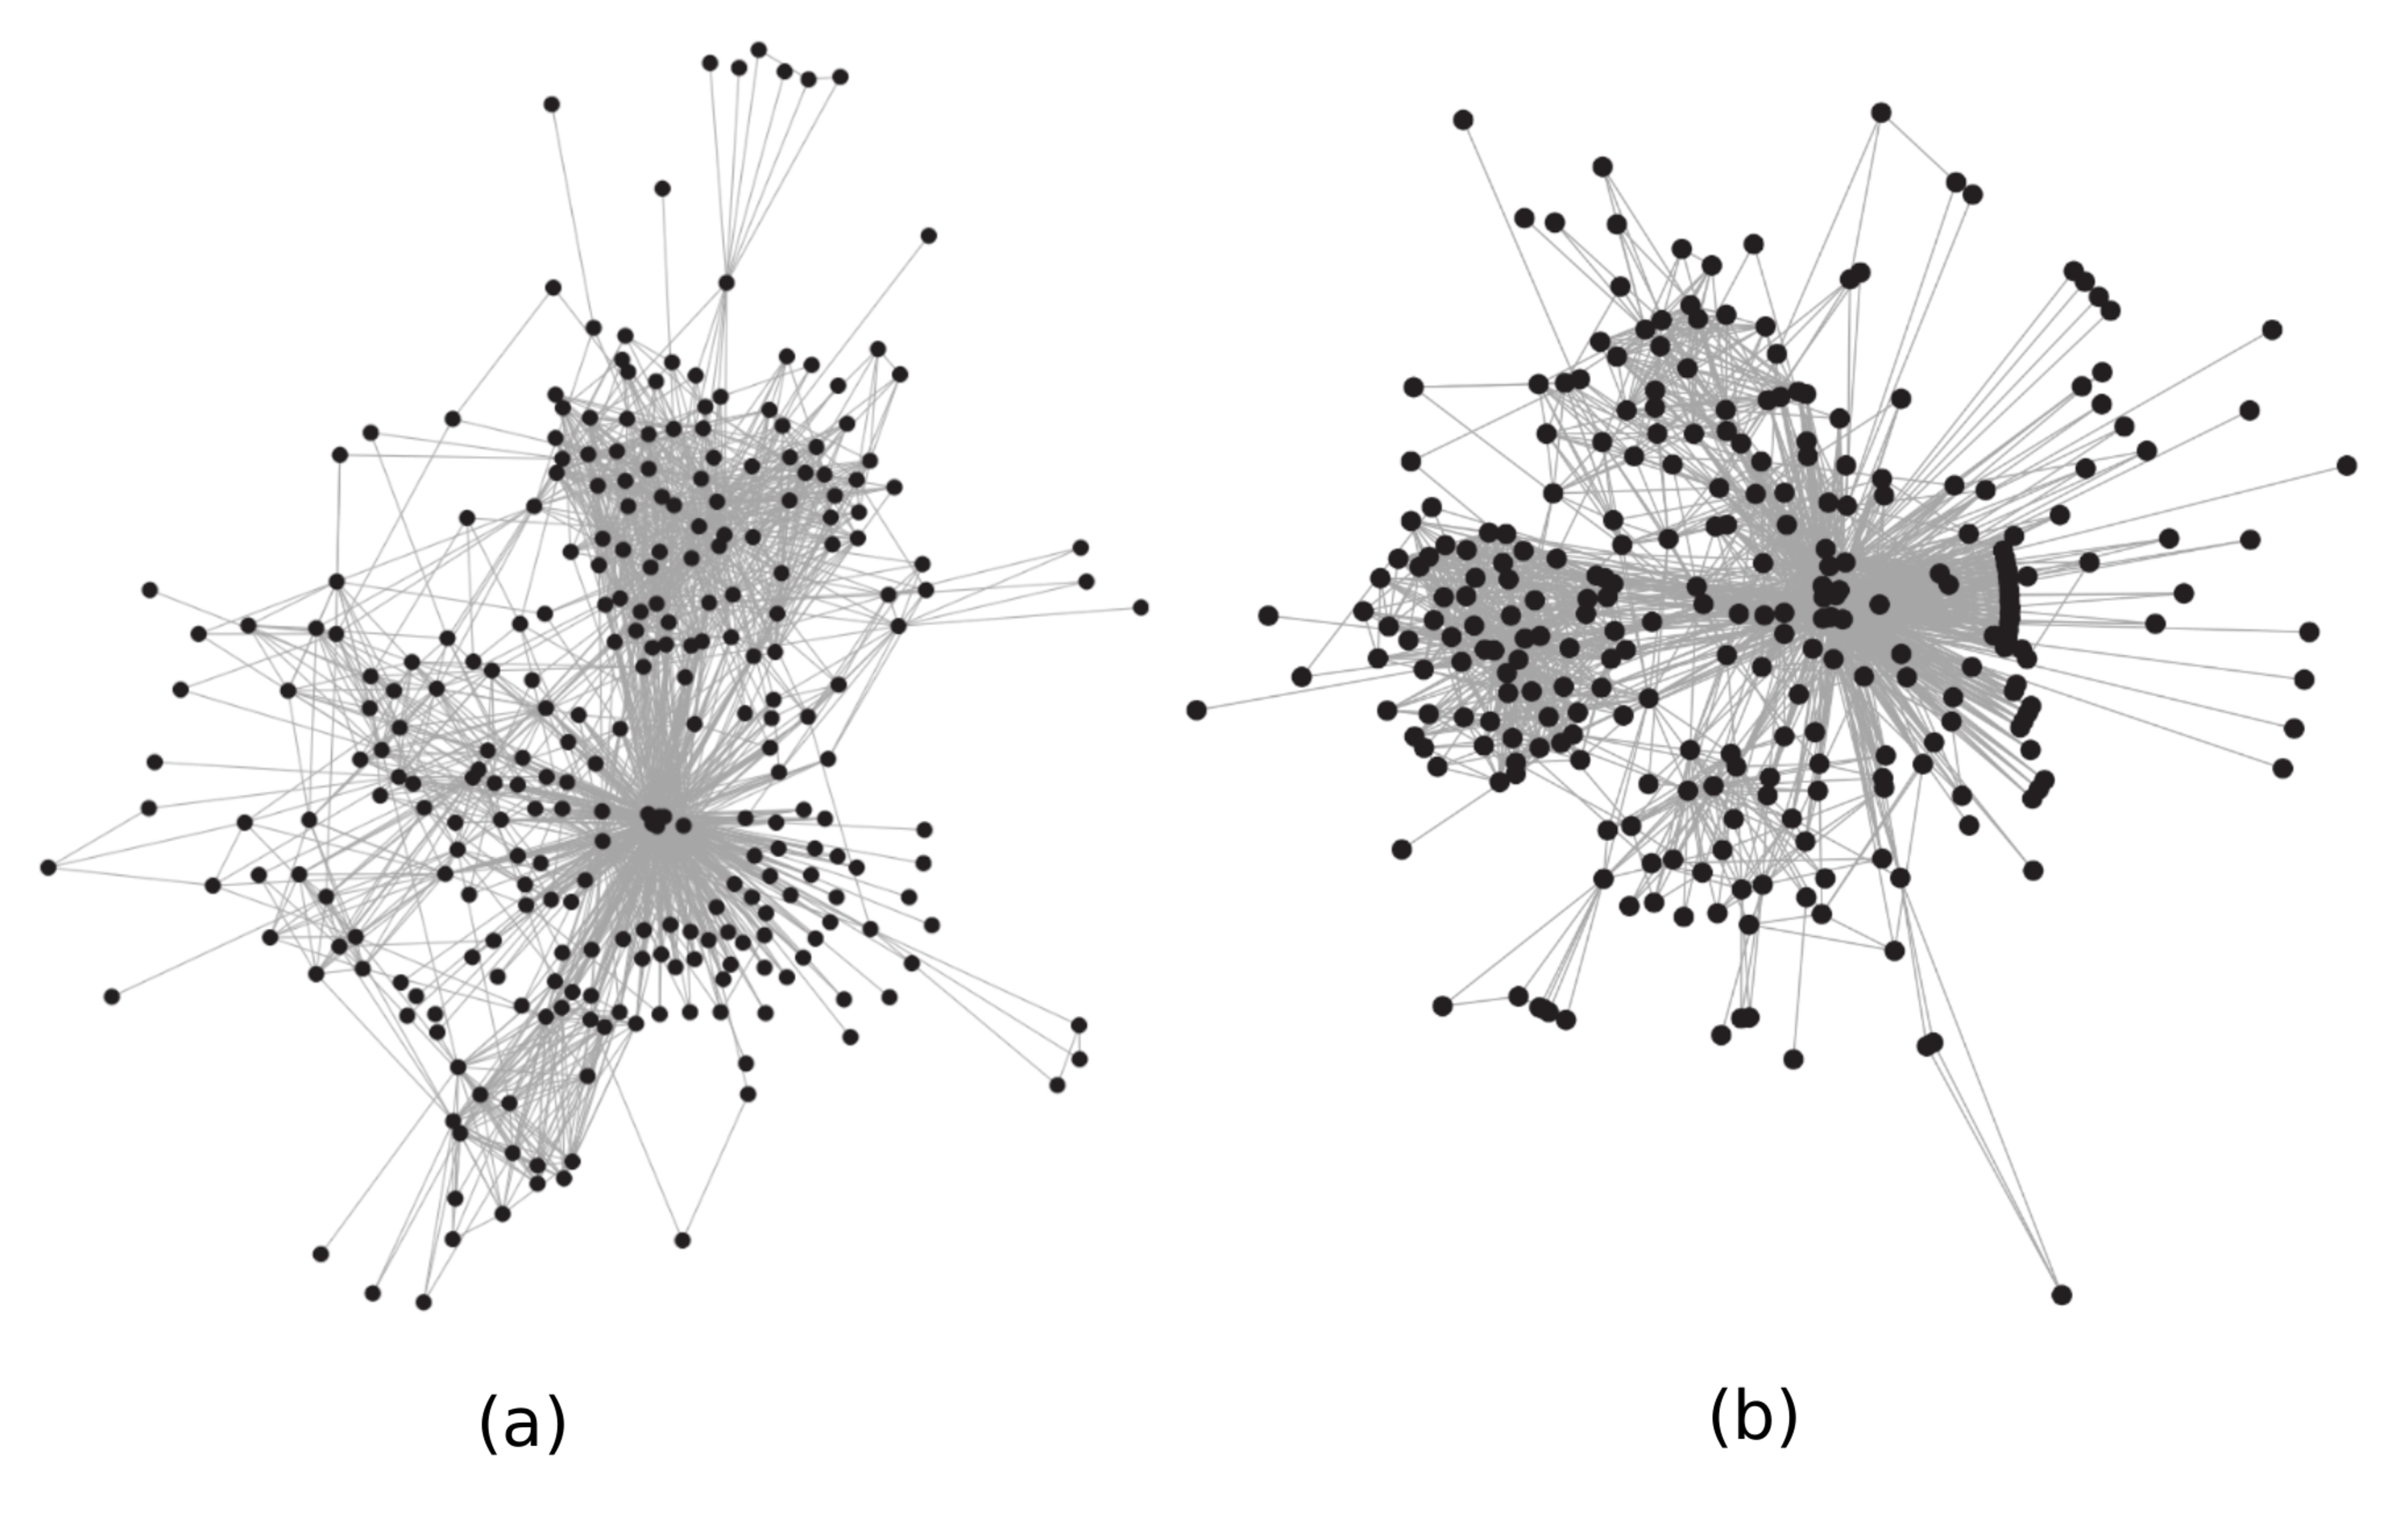
\includegraphics[scale=0.16]{media/layout_techniques.pdf}
    \caption{The protein interaction network laid out using the graph embedder (GEM) (a) and Kamada and Kawai's algorithm (b). Modified from \cite{Gibson2013}.}
    \label{fig:layout_techniques}
\end{figure}
\subsection{Layout Techniques}
One of the oldest and most established classes is the family of force-based layouts. In this class spring-electrical and energy based approaches have to be distinguished.\\ 
The first type makes use of Eades' spring-embedder \cite{Gibson2013}, meaning that nodes are modeled as steel rings and edges as springs. Connected nodes attract each other while all other nodes repel. After initializing the system with a random state, the attracting and repulsive forces and the system's temperature are repeatedly calculated to update node positions until the system reaches an equilibrium. Although this approach was only intended to work for small graphs (< 50 nodes), many adaptions have been made that tried to improve both run-time and the resulting layout. Among other adaptions, for instance, Fruchterman and Reingold\cite{Fruchterman1991} sped up their algorithm by only considering neighbouring nodes within a certain radius for the force calculation and the graph embedder algorithm (GEM) additionally considered gravitational forces and moreover introduced a local temperature that determines how far a node can travel in a single iteration \cite{Gibson2013}.\\
Energy based approaches also utilize Eades' spring-embedder but consider the layout task as an optimisation problem in which an energy function that contains the desired properties of the layout has to be minimized \cite{Gibson2013}. For Example Kamada and Kawai \cite{Kamada1989} try to approximate the layouts' Euclidean distance with their graph-theoretic distance (the shortest path length between two vertices). Symmetry is the main goal of their approach and consequently their cost function measures the lack of it.
Visual examples for the mentioned algorithms can be found in \autoref{fig:layout_techniques}.\\
Despite the various adaptions and run-time improvements, this class of algorithms still isn't suited for large and dense graphs.\cite{Gibson2013} \cite{VonLandesberger2011}.
\\
Constraint-based layouts extend the idea of force based approaches. They allow the user to define constraints such as closeness of groups, node alignment along an axis, edge direction etc. This enhances the power of expression but exacerbates the run-time issue of the underlying force-based approach\cite{VonLandesberger2011}.


Another category is multiscale algorithms. The core idea is to hierarchically decompose a graph into smaller sub-graphs and iteratively add nodes to an initially rough structure. These algorithms differ in their graph decomposition and layer layouting technique. For instance Muelder and Ma \cite{Muelder2008} used clustering for decomposition and space filling curves for the layout, which resulted in short run-times and comprehensible layouts even for dense graphs. Typically this class of algorithms is significantly faster than force-based techniques\cite{VonLandesberger2011}. \\
Besides these rather established techniques also non standard algorithms such as dimension reduction approaches can be used to generate layouts. This type of algorithm tries to map information that's expressed in a high-dimensional space onto a mostly 2 or 3 dimensional space. The preservation of relevant information has to be guaranteed as far as possible during this reduction. For this cause, the graph-theoretic distance between node pairs is often used as the information to be saved. While layouting graphs fast, the produced layouts' quality highly depends on the graph's structure and is quite sensitive, meaning that small structural modifications significantly influence the layout's quality \cite{Gibson2013} \cite{VonLandesberger2011}.

\begin{figure}
    \centering
    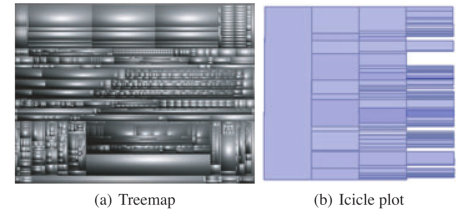
\includegraphics{media/space_filling_trees.pdf}
    \caption{Examples for space filling tree visualizations while using the principle of a) enclosure and b) adjacency. Taken from \cite{VonLandesberger2011}.}
    \label{fig:space_filling_trees}
\end{figure}

All previously introduced techniques work on general graphs. However, in certain use-cases graphs have a specific structure that allow specialized techniques to produce high quality layouts with reduced complexity. For instance, file systems or taxonomies are typically represented as a tree. Trees can be visualized with node-link diagrams exemplary in 2D using layered, radial or balloon layouts, in 3D with cone trees or with hyperbolic layouts. Herman et al. provides an overview of the mentioned techniques \cite{Herman2000}. Most of them have a linear complexity in time and memory which makes them extremely scalable and hence preferable to general layout techniques if applicable. \\
In addition to the node-link visualizations especially trees can also be displayed with space-filling techniques. These try to make use of the entire space and utilize e.g. the principle of enclosure (recursively layout children within the area of the parent, \autoref{fig:space_filling_trees}a) or adjacency (place children next to parents without overlapping, \autoref{fig:space_filling_trees}b) to display edges instead of links\cite{VonLandesberger2011}.



\section{Complexity Reduction}
No matter how good a layout is - if a graph contains thousands or even millions of nodes and edges it gets extremely hard to understand its structure and extract valuable information. For this purpose different complexity reduction techniques can be applied that either highlight relevant information or remove details for the sake of an better overview. A selection of such techniques will be presented in this following section.

\subsection{Pre-processing}
Before using a layout technique on a graph, pre-processing algorithms are often applied to simplify the graph while preserving its core structure. These simplifications can usually be performed autonomously without user interaction and come in two main forms: Graph filtering and graph aggregation \cite{VonLandesberger2011}.
Graph filtering can be either stochastically, which means that nodes and edges are mainly removed randomly, or deterministically. Deterministic algorithms also remove nodes and edges but make these decisions based on node or edge attributes, topological values or other graph properties.\\
Graph aggregation on the other hand does not remove nodes and edges but merges them and thereby reduces size and complexity. This aggregation step can be applied multiple times to generate different levels of detail of the same graph. The selection process of nodes that will be aggregated is usually based on attributes, clusters or known hierarchies \cite{VonLandesberger2011}.

\begin{figure}
    \centering
    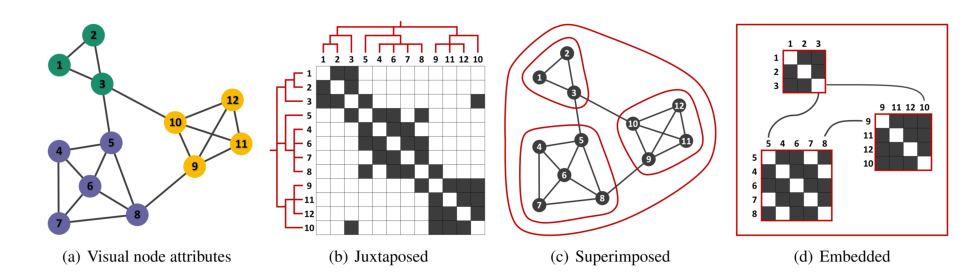
\includegraphics[scale=0.5]{media/group_vis.pdf}
    \caption{Different grouping techniques for the same graph. (a) Visual node attributes - here color. (b) Juxtaposed - here using an attached approach. (c) Superimposed - here using a contour approach. (d) Embedded - here using a hybrid approach. Taken from \cite{Vehlow2015}.}
    \label{fig:group_vis}
\end{figure}
\subsection{Grouping}
Another highly useful way of reducing complexity is to highlight group structures to provide an better overview of the data. For this purpose Vehlow et al.\cite{Vehlow2015} propose four main visualization types: Visual node attributes, Juxtaposed, Superimposed and Embedded.\\
The first technique, called 'visual node attributes', uses the nodes visual representation properties to encode its association with one or multiple groups ( \autoref{fig:group_vis}a). Regardless of the fact that humans can't easily distinguish more than 7 colors \cite{Healey1996}, node coloring is often used to link vertices to groups. Different techniques try to optimize the color selection by either maximizing color differences between neighbouring groups or assigning similar colors to similar groups. Visualizing groups via visual node attributes is commonly combined with other approaches that will be introduced in the following.\\
Techniques that display the graph and its group structure adjacently are referred to as juxtaposed approaches (\autoref{fig:group_vis}b). In this category, one has to further differentiate between attached and separate visualizations. Attached visualizations directly connect to the graph representation and are usually applied to adjacency matrix visualizations. Even tough they can be applied to node-link diagrams, if the nodes are aligned along one axis, this condition makes the approach unsuitable for large node-link representations.
Separate juxtaposed visualizations are more appropriate for node-link diagrams. They visualize the group structure in a separate view and then connect the both representations via visual indicators, like e.g. color or links, or interaction.\\
Superimposed approaches render an additional layer on top of the graph visualization that is aligned with the underlying node-link diagram. To illustrate the groups one of three categories can be used: Line overlay methods draw a continuous line between all nodes of each group. In order to reduce cluttering, the lines can, for example, be minimized by applying an adapted travelling sales man heuristic \cite{Alper2011}. Contour overlays on the other hand draw closed contours that can differ in shape. All nodes within a contour are considered to be part of the group that is represented by the respective surrounding shape.
The last type, Partitioning, is contrarily to the previous technique a space filling approach that decomposes the area into sections. Each of these section behaves identically to the contour idea by associating nodes with groups through visual enclosing. All introduced superimposed techniques can be combined with coloring (\autoref{fig:group_vis}c).\\
Lastly groups can be visualized through embedding. This means that groups are also modelled as nodes and are a part of the graph (\autoref{fig:group_vis}d). Beside the standard node-link diagram, a hybrid node-link and matrix representation can be useful for this technique \cite{Vehlow2015}.\\

\subsection{Edge Bundling}
The last here presented complexity reduction technique is called edge bundling. The main idea is to spatially group similar graph edges to reduce clutter and provide an better overview. Techniques for 3D graphs and also special graphs such as compound graphs exist. However, the following section will focus only on general two dimensional graphs and provide an overview of common techniques and challenges.

\subsubsection{Bundling Techniques}
Basis of most bundling techniques is a so-called compatibility function, typically named $\kappa$ that measures how dissimilar paths are, meaning that low values of $\kappa$ correlate to similar paths and vice versa. Defining a good compatibility function that both considers the layouts spatial and the graphs attribute information is challenging. Moreover, edge bundling techniques have to be differentiated between directed an undirected graphs\cite{Lhuillier2017}.

\paragraph*{Undirected Graphs} Undirected graphs are a common type for graph bundling algorithms. One of the first approaches was force-directed edge bundling (FDEB). It defines $\kappa$ only with respect to geometric information of the edge drawing. This basic technique was soon extended by Ngyuen et al. \cite{Nguyen2011} to also consider topology as well as attributes and therefore importance-based compatibility. While this modification grants more control about the bundling selection it still has no explicit control mesh. A control mesh is a set of control points that determines the rough structure of the resulting edges and thereby enables even more control about the resulting graph representation. A progression based on control meshes proposed by Luo et al. \cite{Luo2012} can help to deal with common bundling issues like difficult end-to-end edge tracing or closeness of bundled edges to unrelated nodes. They achieve this by adapting $\kappa$ to be non-null only for edges that share a node and are close in the base drawing. Moreover, edges are repelled from unrelated nodes. While this extension eases edge tracing for small graphs (< 100 nodes and edges) it often fails to sufficiently reduce clutter for larger graphs with thousands of nodes and edges.\\
All previously presented techniques have issues with large graphs either due to run-time (FDBE, \cite{Nguyen2011}) or insufficient clutter reduction (\cite{Luo2012}). MINGLE \cite{Gansner2011} tackles these issues by introducing a computationally-scalable ink-saving principle that tries to minimize the theoretically used ink to draw edges by using a greedy algorithm that merges close edges as long as it saves ink. This allows bundling for graphs with up to a million edges with the drawback of creating less smooth results \cite{Lhuillier2017}. 

\paragraph*{Directed Graphs}  A common criticism of general bundling techniques is that they ignore the semantic carried by edge directions even though this information can be vital for certain applications such as exploring a software system's call graph. The additional information of direction can be easily added by coloring edges with a source to destination color gradient. However, this leads to color mixing problems when edges of different directions are bundled \cite{Lhuillier2017}. To fix this problem, techniques specifically for directed graphs have been introduced that add the edge direction to the compatibility function $\kappa$. An example algorithm for directed edge bundling is Divided Edge Bundling (DEB)\cite{Selassie2011}, which can be seen as an extension of FDEB that takes edge direction into account. Among other modifications, it adds repulsion of opposing edges and includes edge weight into $\kappa$ to reduce bundling of important edges. This method produces good results for directed graphs but claims more space and produces more clutter compared to FDEB. A direct comparison between both approaches can be found in \autoref{fig:airline_edge_bundling} \cite{Lhuillier2017}.\\


\begin{figure}
    \centering
    \includegraphics[scale=0.9]{media/airline_edge_bundling.pdf}
    \caption{Comparison of a general bundling algorithm (FDEB, a) and a bundling algorithm for directed graphs (DEB, b) applied on the US airlines graph ($|V| = 235, |E| = 2101$). Taken from\cite{Lhuillier2017}.}
    \label{fig:airline_edge_bundling}
\end{figure}


\subsubsection{Bundling Visualizations}
After applying a bundling technique the bundled data can be visualized and even further improved using different techniques such as blending, data color mapping, shading or smoothing and deformation.\\
Blending deals with overlapping edges and eases the readability of connection strength and amount of paths between endpoints. This is achieved by rendering dense bundles more opaque than sparse ones by mapping the local bundle density to visual properties like opacity, color or shading (\autoref{fig:blending}) \cite{Lhuillier2017}.\\
Data color mapping maps edge attributes to colors. As already seen in section 3.3.1 - directed graphs, this attribute could be direction but moreover also spatial density or domain specific attributes like for example the local flight height for the us airline example. As mentioned earlier overlapping paths provoke a color mix issue for which no general solution exists so far.
To further emphasize important connections, shading can be used. For instance, a false height map that is increasing parabolically from a bundles border to its center can be defined. This map is then processed by a shading algorithm, making crossing edges easier to distinguish. This is often combined with color mapping.
Finally bundled edges can also be smoothed, commonly achieved by applying Laplacian smoothing, or deformed in order to avoid landmarks in the drawing space. The latter can be accomplished e.g. by making the landmarks repulsive, which can both be applied during the bundling iterations or as a post-processing step \cite{Lhuillier2017}.

\begin{figure}
    \centering
    \includegraphics[scale=0.9]{media/blending.pdf}
    \caption{A graph drawn with opacity blending (right) and without (left). Taken from \cite{Lhuillier2017}.}
    \label{fig:blending}
\end{figure}
\begin{figure}
    \centering
    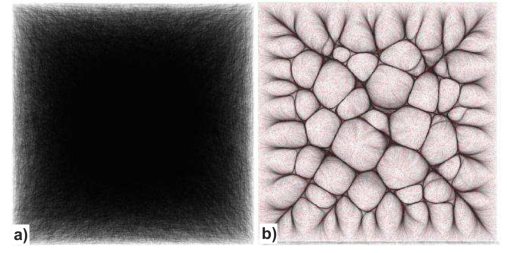
\includegraphics[scale=0.7]{media/faithfullness_bundling.pdf}
    \caption{A pseudo-random graph visualized without simplification (a) and an exemplary bundling (b). Taken from \cite{Lhuillier2017}.}
    \label{fig:faithfulness}
\end{figure}
\subsubsection{Bundling Challenges}
In addition to the already discussed difficulties of bundling, a few other general challenges like quality, faithfulness and control have to be mentioned.
In general, it is quite hard to define what qualifies a bundling as good. Although certain criteria such as ink-minimization, edge crossings, faithfulness and more have been discussed, no such set of metrics entirely covers edge bundling\cite{Lhuillier2017}. 
Moreover, edge bundling techniques have to be evaluated on how much information is lost during the process and also if wrong information is added. For instance, bundling techniques can visualize non-existent structures in a pseudo-random graph (\autoref{fig:faithfulness}).
Lastly, due to advances in the field, bundling techniques nowadays have a lot of parameters that are often coupled. This aggravates the recreation of graphs for users after switching techniques \cite{Lhuillier2017}.\\
Despite multiple general complexity reduction techniques, resulting graph layouts often still don't fit a user's specific need. 
For this purpose, a range of user interaction techniques exists that enable the user to further enhance the visualization and interact with it. A selection of such approaches will be presented in the following. 

\begin{figure}
    \centering
    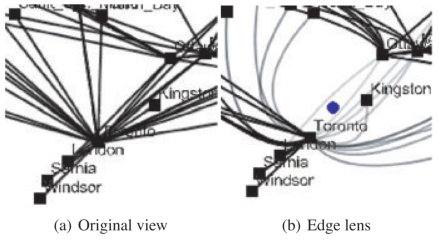
\includegraphics[scale=0.8]{media/edge_lense.pdf}
    \caption{Example of edge lens interaction. (a) Original view without lens. (b) Using edge lens. Taken from \cite{VonLandesberger2011}.}
    \label{fig:edge_lense}
\end{figure}
\section{User Interaction}
The most traditional tools of user interaction are zoom and pan. Zooming can take two forms: Geometric zooming simply blows up the graph content while semantic zooming also changes the content by adding details\cite{Herman2000}. To generate different level of detail for the latter, aggregation techniques as described in section 3.1 can be used. Panning on the other hand allows the user to translate the plot to different viewpoints in a zoomed in graph. For node-link diagrams panning is often implemented to move along the graph's edges (guided panning) to properly explore the graph's structure \cite{VonLandesberger2011}.\\ 
While zooming can help to focus on a specific part of the data, contextual information is lost in the process, which makes it hard to fully understand the displayed information. To solve this issue a technique often referred to as magic-lense \cite{VonLandesberger2011} or focus+context \cite{Herman2000} can be used. The main idea is to highlight an area of interest by assigning more space to the data within it and distorting the surrounding. This idea can be applied to node-link diagrams as well as space-filling techniques and also allows the user to select multiple areas of focus. For geometric changes this technique is called fisheye views \cite{VonLandesberger2011}. These so-called lenses can be either applied to the entire graph data within the selected area or just the edges (edge lenses). Edge lenses help to declutter strongly overlapping edges in graphs that try to minimize node repositioning (e.g. geographic-based graphs as in \autoref{fig:edge_lense}). Other approaches use edge-filtering in the focused area or move neighbouring nodes closer to a highlighted vertex.\\
In addition to modifying the final result of a graph visualization, users can also adjust the underlying visualization type and its parameters. Typical changes to visual parameters are highlighting of interesting items, which is often synchronized across multiple views of the same graph, or changes to the visual schemes layout or representation. Layout adaptions can be either changes to the layout type that are followed by an automatic recalculation or manual movement of nodes. User can also select a different visual representation, e.g. switching from a node-link diagram to a matrix representation, which can provide new insights. If applicable, smooth animations should be used to make the transformations comprehensible \cite{VonLandesberger2011}.


\section{Conclusions}
Graph layouting is a challenging topic that made significant progress within the last decades. It is used in areas such as biology, social network analysis and more and contributes to extracting useful information from huge sets of graph structured data. This paper collated information from various research and provided a brief overview of graph representation types and introduced different categories of layouting techniques. Moreover multiple approaches to reduce a graphs complexity, namely pre-processing steps like filtering and aggregation, grouping methods and especially edge bundling techniques and their visualizations and challenges have been presented. Lastly, different user interaction methods have been discussed. Although recent techniques have become more scalable, this process needs to continue to enable the analysis of the data sets that keep growing. However, approaches still need to remain usable in practice by limiting their usage complexity to a reasonable level.
%layouting and complexity reduction techniques as well as different user interaction possibilities by collating information from prominent research.


%-------------------------------------------------------------------------

%\bibliographystyle{eg-alpha}
\bibliographystyle{eg-alpha-doi}

\bibliography{references}

%-------------------------------------------------------------------------


\end{document}

